\noindent
\includegraphics[height=1.25cm]{images/pictograms/replication}
\includegraphics[height=1.25cm]{images/pictograms/under_construction}
\includegraphics[height=1.25cm]{images/pictograms/msc}

%%%%%%%%%%%%%%%%%%%%%%%%%%%%%%%%%%%%%%%%%%%%%%%%%%%%%%%%%%%%%%%%%%%%%%%%%%%%%%%%%%%%%%%%%%%%%%%%%%%

\begin{flushright} {\tiny {\color{gray} python\_codes/fieldstone\_167/text.tex}} \end{flushright}

%\lstinputlisting[language=bash,basicstyle=\small]{python_codes/template_keywords.key}

\par\noindent\rule{\textwidth}{0.4pt}

\begin{center}
\inpython
{\small Code: \url{https://github.com/cedrict/fieldstone/tree/master/python_codes/fieldstone_167}}
\end{center}

\par\noindent\rule{\textwidth}{0.4pt}

{\sl This stone was developed in collaboration with Daniel Cayuela-Barcham and Alissa Kotowski}. 
\index{contributors}{A. Kotowski}
\index{contributors}{D. Cayuela-Barcham}

\par\noindent\rule{\textwidth}{0.4pt}

%%%%%%%%%%%%%%%%%%%%%%%%%%%%%%%%%%%%%%%%%%%%%%%%%%%%%%%%%%%%%%%%%%%%%%%%%%%%%%%%%%%%%%%%%%%%%%%%%%%

This \stone takes its origin in the MSc work of Daniel about the subduction interface. 
\textcite{stuw98} (1998) proposes a simple mathematical model for the influence 
of shear heating on the temperature there, so it was decided to 
reproduce the results of the paper (esp. Fig.~6) and use it as a basis for discussion.


%-------------------------------------------------
\subsection*{Theory}

We start with the heat transport equation where the advection and diffusion terms 
are assumed to be negligible and the only source of heat would come from the shear heating:
\[
\rho C_p \frac{dT}{dt} = H_s = \sum_{ij}\sigma_{ij} \dot{\varepsilon}_{ij} = 
{\bm \sigma} : \dot{\bm \varepsilon}
\]
where $H_s$ is the volumetric rate of shear heat production, 
$\sigma_{ij}$ is the stress tensor and  $\dot{\varepsilon}_{ij}$ the strain rate tensor.

In order to do our estimates on the simplest level, a deformation
geometry of biaxial horizontal compression is assumed where the off-diagonal terms of the strain rate
tensor as well as $\dot{\varepsilon}_{yy}$ are zero and $\dot{\varepsilon}_{xx}=-\dot{\varepsilon}_{zz}
=\dot{\epsilon}$ (thereby implying that the trace of the tensor is zero, i.e. the flow
is incompressible).

Concretely, the strain rate tensor (in the right coordinate system) can then be written:
\[
\dot{\bm \varepsilon} = 
\left(
\begin{array}{ccc}
\dot\epsilon &0 & 0 \\
0 &0 & 0 \\
0 & 0 & \dot\epsilon
\end{array}
\right)
\]
with the second invariant thereof given by
\[
{\cal I}_2(\dot{\bm \varepsilon}) 
= \frac12 \dot{\bm \varepsilon}:\dot{\bm \varepsilon}
= \frac12 (
\dot\varepsilon^2_{xx} + \dot\varepsilon^2_{yy} + \dot\varepsilon^2_{zz}
)+ 
\dot\varepsilon^2_{xy} + \dot\varepsilon^2_{xz} + \dot\varepsilon^2_{yz}
=\frac12 ( \dot\epsilon^2 + \dot\epsilon^2)
= \dot\epsilon^2
\]

In this deformation geometry, the principal stresses ($\sigma1$ and $\sigma_3$ correspond 
to the horizontal and vertical stresses and there is no shear stress so that 
the mean stress can be expressed as $\tau = \frac12(\sigma_1-\sigma_3)$.

For this, we assume the form suggested by \textcite{brko80} (1980) 
(St\"uwe probably refers to their Eq.~4)
which includes the exponential dependence of stress on temperature:
\[
\tau = \frac{1}{2} (\sigma_1-\sigma_3) = \frac12 \left(\frac{\dot\varepsilon}{A} \right)^{1/n}
\exp \left( \frac{Q}{nRT} \right)
\]
which leads to write :
\[
{\bm \tau} = \frac12 \left(\frac{\dot\epsilon}{A} \right)^{-1+1/n}
\exp \left(\frac{Q}{nRT} \right) \dot{\bm \varepsilon}
\]
where $A$ and $Q$ are the pre-exponent constant and activation energy, $n$ is the power law exponent, 
which is assumed to be 3, and $R$ is the gas constant.

We have ${\bm \sigma} = - p {\bm 1} + {\bm \tau}$, where ${\bm \tau}$ is the 
deviatoric stress tensor so that the shear heating term writes
\begin{eqnarray}
{\bm \sigma}:\dot{\bm \varepsilon} 
&=& - p \underbrace{{\bm 1}:\dot{\bm \varepsilon}}_{= Tr({\bm \dot\varepsilon})=0} + {\bm \tau}:\dot{\bm \varepsilon} 
\; = \; \frac12 \left(\frac{\dot\epsilon}{A} \right)^{-1+1/n}
\exp \left(\frac{Q}{nRT} \right) \underbrace{\dot{\bm \varepsilon}: \dot{\bm \varepsilon}}_{2 \dot\epsilon^2}
\end{eqnarray}
so that in the end:
\[
\boxed{
\frac{dT}{dt} = \frac{\dot\epsilon}{\rho C_p}  \left(\frac{\dot\epsilon}{A} \right)^{1/n}
\exp \left(\frac{Q}{nRT} \right)
}
\]
which is Eq.~(6) of \textcite{stuw98} (1978)\footnote{Save for factor 2. However note that this factor 2 
disappears in Eq.~7 so which one is it?}

In order to solve this ODE we follow the same procedure as in the appendix of the paper. 
Assuming the strain rate $\dot\epsilon$ to be constant, we define 
\[
C = \frac{\rho C_p}{ \dot\epsilon} \left(\frac{\dot\epsilon}{A} \right)^{-1/n}
\qquad
\text{and}
\qquad
D = \frac{Q}{nR}
\]
so that now
\begin{eqnarray}
\frac{dT}{dt} &=& C^{-1} e^{D/T} \nn\\
\Rightarrow C e^{-D/T}  dT &=&  dt \nn\\
\Rightarrow \int_{T_0}^{T_f} C e^{-D/T}  dT &=&  \int_0^t dt 
\end{eqnarray}
where we have integrated between the limits of temperature at the start of
deformation, $T_0$, and temperature at the end of deformation $T_f$.
We then obtain 
\[
t = C \int_{T_0}^{T_f} e^{-D/T}  dT
\]
We carry out a simple change of variable: $x=D/T$, so that $dx = -\frac{D}{T^2} dT$ 
and also $dT=-\frac{D}{x^2} dx$. Then 
\[
t = C \int_{x_0}^{x_f} e^{-x} \left(-\frac{D}{x^2} \right) dx 
= CD \int_{x_0}^{x_f} \left(-\frac{1}{x^2} \right) e^{-x} dx
\]
where $x_0=D/T_0$ and $x_f=D/T_f$. There probably is a minus sign missing in Eq.~9.

The integral in the rhs can be integrated by parts\footnote{$\int u'v = uv - \int uv'$}:
\[
\int_{x_0}^{x_f} \left(-\frac{1}{x^2} \right) e^{-x} dx 
=  \left[\frac{1}{x} e^{-x} \right]_{x_0}^{x_f} - \int_{x_0}^{x_f} \frac{1}{x} (-e^{-x}) dx
= \frac{e^{-x_f}}{x_f}  - \frac{e^{-x_0}}{x_0}  +
\int_{x_0}^{x_f} \frac{1}{x} e^{-x} dx
\]
The integral in the rhs is close to the so-called 
exponential integral\footnote{\url{https://en.wikipedia.org/wiki/Exponential_integral}}
$\text{Ei}$ defined as follows:
\[
\text{Ei}(x)= - \int_{-x}^\infty \frac{e^{-t}}{t} dt 
\qquad \text{or,} \quad
\text{Ei}(-x)= -\int_{x}^\infty \frac{e^{-t}}{t} dt
\]
The second expression will prove useful in what follows.
Using Eq.~12 of \textcite{stuw98}: 
\begin{eqnarray}
\int_{x_0}^{x_f} \frac{ e^{-x}}{x}  dx
&=& \int_{x_0}^\infty \frac{e^{-x}   }{x}  dx + \int^{x_f}_\infty \frac{e^{-x}}{x}  dx \nn\\
&=& \int_{x_0}^\infty \frac{e^{-x}   }{x}  dx - \int_{x_f}^\infty \frac{e^{-x}}{x}  dx \nn\\
&=& -\text{Ei}(-x_0) + \text{Ei}(-x_f)
\end{eqnarray}
we arrive at 
\[
\boxed{
t= CD \left[
\frac{e^{-x_f}}{x_f}  - \frac{e^{-x_0}}{x_0}  
+ \text{Ei}(-x_f) -\text{Ei}(-x_0) 
\right]
}
\]
There remains a problem: this equation is not identical to Eq.~13 
of the paper:
\begin{center}
\includegraphics[width=6.5cm]{python_codes/fieldstone_167/images/stuw98_eq}
\end{center}


Finally, if we replace time by $t=\epsilon / \dot\epsilon$, assume we set a 
desired value for the strain $\epsilon$, the equation above can be solved numerically for $T_f$:
\[
\frac{\epsilon}{\dot\epsilon} = 
CD
\left[
\frac{e^{-D/T_f}}{D/T_f}  - \frac{e^{-D/T_0}}{D/T_0}  
+ \text{Ei}(-D/T_f) -\text{Ei}(-D/T_0) 
\right]
\]
but for simplicity we will solve it for $x_f$ in that form:
\begin{equation}
\frac{t}{CD}
-
\left[
\frac{e^{-x_f}}{x_f}  - \frac{e^{-x_0}}{x_0}  
+ \text{Ei}(-x_f) -\text{Ei}(-x_0) 
\right]
=0
\label{f167:eqnl}
\end{equation}
This is a nonlinear equation of the form $f(x_f)=0$. We assume a starting temperature $T_0$, 
compute $x_0$, assign material values $\rho,C_p,A,n$, choose a strain rate value $\dot\epsilon$, 
a total strain $\epsilon$ and can then proceed to solve the equation for $x_f$.




When it comes to Ei these must be evaluated numerically, for instance with 
\url{https://docs.scipy.org/doc/scipy/reference/generated/scipy.special.expi.html}
where we see that 
the exponential integral is defined as 
\[
Ei(x) 
= \int_{-\infty} ^x \frac{e^t}{t}dt
= \int_{\infty}^{-x} \frac{e^{-t}}{-t} (-dt)
= \int_{\infty}^{-x} \frac{e^{-t}}{t} dt
= -\int_{-x}^\infty \frac{e^{-t}}{t} dt
\]
which is the standard definition that we have used above.


%-------------------------------------------------
\subsection*{About Fig. 6 of the paper}

Let us consider Fig.~6 of \textcite{stuw98}, where three different sets rheological constants are used
for $A$ and $Q$.

\begin{center}
\includegraphics[width=8cm]{python_codes/fieldstone_167/images/stuw98_fig6}\\
{\captionfont  Taken from \cite{stuw98}.
The curves are labelled for $\log_{10} \dot\epsilon$. 
The rheological data used for the three solid curves are the quartz data of \cite{brko80}:
$A=5\cdot 10^{-6} \si{\per\cubic\mega\pascal \per \second} $, $Q=1.9\cdot 10^5 \si{\joule\per\mol}$
The rheological data
used for the three dashed curves are the average quartz date used
by \cite{stsa94}: $A=2\cdot 10^{-4} \si{\per\cubic\mega\pascal \per \second} $, $Q=2.5\cdot 10^5 \si{\joule\per\mol}$. The data for the dotted curve are the
olivine data of \cite{brko80}: 
$A=7\cdot 10^{4} \si{\per\cubic\mega\pascal \per \second} $, $Q=5.2\cdot 10^5 \si{\joule\per\mol}$. All curves are calculated for
a total strain of one.
}
\end{center}

Obviously the final temperature $T_f$ can not be lower than the initial temperature $T_0$
($H_s\ge 0$) so that the lower left of the figure is not accessible. Also this means that we should
look for the root of Eq.~\eqref{f167:eqnl} in the range $T_f\ge T_0$.

We read:
\begin{displayquote}
{\color{darkgray}
Fig.~6 shows that for reasonable strain rates and strains the temperatures of rocks at 600\si{\celsius} 
may be increased by 100-200\si{\celsius}. 
Colder rocks can heat more, because they can sustain higher shear stresses until
strain heating weakens them (Pavlis, 1986). Importantly, rocks colder than about 500-600\si{\celsius} 
will reach similar temperatures by the effects of strain heating, independently
of their temperature prior to deformation (Pavlis, 1986). Thus, the effects of shear heating
on a large vertical section of the crust may be that
this section is made isothermal.}
\end{displayquote}

Coming back to the figure in the paper, we can add lines to it and 
we then quickly realise that the diagonal line labeled 'no shear stress'
has likely been drawn by hand since it does not follow the $T_0=T_f$ line
indicated in purple:

\begin{center}
\includegraphics[width=7cm]{python_codes/fieldstone_167/drawing.png} \\
{\captionfont Fig 6 of the paper to which horizontal and vertical lines 
have been added.}
\end{center}

%-------------------------------------------------
\subsection*{The python code}

First, we notice that the $A$ values are provided in \si{\per\cubic\mega\pascal \per \second}.
We have 
\[
1~\si{\per\cubic\mega\pascal} = (10^6 \si{\pascal})^{-3} = 10^{-18}~\si{\per\cubic\pascal}
\] 
so that for example $5\cdot 10^{-6}~\si{\per\cubic\mega\pascal\per\second} 
= 5 \cdot 10^{-24}~\si{\per\cubic\pascal \per\second}$.

Second, the gas constant $R$ and the heat capacity $C_p$ are expressed in 
\si{\joule\per\mol\per\kelvin} and \si{\joule\per\kg\per\kelvin} so that 
all temperatures in the equations above must be in \si{\kelvin}.

We first declare all the variables needed:

\begin{lstlisting}
TKelvin=273.
R=8.314
Cp=1000
n=3.
rho=2750
e=1        # total strain
A=5e-24
Q=1.9e5
\end{lstlisting}

We then create an array that contains
temperature values in \si{\celsius} between 400 and 1400:

\begin{lstlisting}
Trange=np.arange(400,1400,1)
\end{lstlisting}

We then create the following function which corresponds to Eq.~\eqref{f167:eqnl}.
Note that the conversion from \si{\celsius} to \si{\kelvin} occurs in the function
so that its arguments \lstinline|T,T0| are in \si{\celsius}:
\begin{lstlisting}
def f(T,T0,D,t):
    TT=T+TKelvin
    x=D/TT
    TT0=T0+TKelvin
    x0=D/TT0
    return  t/C/D - ( np.exp(-x)/x -np.exp(-x0)/x0 -scp.special.expi(-x0) +scp.special.expi(-x) ) 
\end{lstlisting}

We then proceed to loop over three values of strain rate $10^{-13,-14,-15}~\si{\per\second}$and 
for each we compute $C$, $D$ and $t$:

\begin{lstlisting}
for sr in (1e-13,1e-14,1e-15):
    D=Q/n/R
    C=rho*Cp/sr*(sr/A)**(-1./n)
    t=e/sr
\end{lstlisting}

Inside this loop we then loop over all values of \lstinline|T0| and 
evaluate the function for all temperatures of the \lstinline|Trange| array:
\begin{lstlisting}
    for T0 in range (400,1400,1):
        res=f(Trange,T0,D,t)
\end{lstlisting}

The \lstinline|res| array then contains the values of the function for a given \lstinline|T0|.
We must then proceed to find its zero(es), if any. 
Before implementing any kind of algorithm, we may wish to visually confirm 
that the data contained in \lstinline|res| does indeed cross the horizontal axis. 
We therefore set $\dot\epsilon=10^{-14}~\si{\per\second}$ and plot the array 
for a few values of \lstinline|T0|:

\begin{center}
\includegraphics[width=8cm]{python_codes/fieldstone_167/lines/res.pdf}
\end{center}

Let us here not dwell on the actual locations of the zeros (see next section), 
but rather rejoice: The function is monotonous and it looks like there will 
be only a single zero value between 400~\si{\celsius} and 1400~\si{\celsius}. 
At this stage, we could then decide to use a ready-made python function that 
would allow us to find the zero with high accuracy via a Newton-Raphson algorithm, 
but given the first-order nature of the whole exercise, locating the 
zero within one degree is more than sufficient. We have therefore implemented
a very simple algorithm: if two consecutive values inside the \lstinline|res|
array are of opposite sign then the zero lies there and the corresponding 
temperature value is written to file next to the \lstinline|T0| value. 
This translates as follows:


\begin{lstlisting}
for sr in (1e-13,1e-14,1e-15):
    ...
    srfile=open('sr'+str(sr)+'.ascii',"w")
    ...
    for T0 in range (400,1400,1):
        ...
        for i in range(0,len(Trange)-1):
            if res[i]*res[i+1]<0: 
               srfile.write("%e %e \n" %(Trange[i],T0))
\end{lstlisting}

In the end the code produces three files
\verb|sr1e-13.ascii|, \verb|sr1e-14.ascii|, and \verb|sr1e-15.ascii|, 
which we can plot in a similar fashion as in Fig.~6 of the paper. 
Actually, as we will see, it will be beneficial to 
also run $\dot\epsilon=10^{-12,-16}~\si{\per\second}$.



%-------------------------------------------------
\subsection*{Results}


Running our code for temperatures between 400~\si{\celsius} and 1400~\si{\celsius}
we arrive at the following temperature profiles for three values of strain rate 
$10^{-13,-14,-15}~\si{\per\second}$:

\begin{center}
\includegraphics[width=5.7cm]{python_codes/fieldstone_167/1kelvin/fig6.pdf}
\includegraphics[width=5.7cm]{python_codes/fieldstone_167/2kelvin/fig6.pdf}
\includegraphics[width=5.7cm]{python_codes/fieldstone_167/3kelvin/fig6.pdf}\\
{\captionfont From left to right: Quartz \cite{brko80}, quartz \cite{stsa94}, olivine \cite{brko80}.}
\end{center}

I have digitized\footnote{\url{https://plotdigitizer.com/app}} the lines of Fig.~6
and these are also plotted on the figures.
This is rather puzzling because our results do not come close to those of Fig~6 at all. 
However, although it is obviously wrong, we could run our code and choose not 
to convert temperatures to \si{\kelvin} (simply by setting \lstinline|TKelvin=0| in the code) 
and we obtain the following figures:

\begin{center}
\includegraphics[width=5.7cm]{python_codes/fieldstone_167/1zero/fig6.pdf}
\includegraphics[width=5.7cm]{python_codes/fieldstone_167/2zero/fig6.pdf}
\includegraphics[width=5.7cm]{python_codes/fieldstone_167/3zero/fig6.pdf}\\
{\captionfont From left to right: Quartz \cite{brko80}, quartz \cite{stsa94}, olivine \cite{brko80}.}
\end{center}

This is rather worrying because these plots do resemble the Fig.~6 of the paper a lot.
We can also try to use Eq.~13 of the paper, implemented in the \lstinline|fstuwe|
function but to no avail.
Also, we find that the lines in the paper are probably for strainrates 
$\dot{\epsilon}=10^{-16,-15,-14}~\si{\per\second}$ unlike stated on the figure of the paper.








